\chapter{Auctions}
\label{sec:auctions}

A Dutch auction works by setting a high starting price, and gradually lowering the price until someone stops the bid. This system has been modelled on that concept, but in reverse. I call it a reverse Dutch auction. \\

The system could have been implemented with workers successively bidding lower for each job, but it was decided that this could mean workers were consistently paid less than they should fairly receive. \\

Each report has a set of Reportables. If any of these Reportables is marked as urgent, an ``urgent" auction is started. Otherwise, the Reportables are placed in a queue, and fed slowly into the system to ensure there is always a job on offer. \\

To configure how an urgent auction is run, an administrator can set the length of time they prefer the job to be in the system. They can do the same for a non-urgent job. The system uses these times to calculate an strategy to minimise the cost to the council. \\

~\cite{dutch} is a paper on optimising Dutch auctions. As this is a reverse Dutch auction, the method in the paper has been altered to reflect this. \\

The jobs in the auctions are ReportedIssues. When an administrator defines Reportables, he also defines the minimum and maximum costs. When a report is made, these costs are used in the auction. \\

Many proofs in~\cite{dutch} require an initial high price, $c_0$, which is gradually lowered until a bidder bids, or it hits a minimum price, $c_{min}$. \\

So as to not have to reprove everything, my reverse auction has been changed to reflect this format. The 
initial price of a job is therefore the negative of the minimum price of the issue. $c_{min}$ is the negative of the maximum price of the issue.

For example, if an issue has a minimum price of £3 and a maximum price of £5, $c_0$, is -3, and $c_{min}$ is -5. When displayed to the user, the prices will be displayed as positive, so it appears to them as if the price is rising. \\

The paper does not specify that $c_0$ nor $c_{min}$ must be positive. \\

The price of an item is kept constant for a fixed interval until the next iteration. At iteration $k$, the price is lowered to $c_k$, where $c_{min} \le c_k \le c_{k-1}$. The auction lasts for $M + 1$ iterations, where $M$ is pre-set by the administrator. \\

As workers must be registered with the system, $n$, the number of bidders, is known. $n$ is assumed constant throughout the auction. Let $X_i$ be bidder $i$'s valuation. The valuations of the $i^{th}$ bidder's values are assumed to be drawn from a known distribution. Let $Y = \max(X_1, X_2, ..., X_n)$ be the maximum valuation of all bidders. Let $F(Y)$ and $f(Y)$ denote the \gls{cdf} and the \gls{pdf}, respectively, of $Y$. \\

Assume $f(Y)$ is a continuous positive function in the range $c_{min}, c_0$. The final payment on the job depends directly on the bidder's maximum valuations, so we can work with $Y$. If the current selling price $c_k$ is lower than $Y$, then at least one worker will immediately bid for the job and end the auction. If $c_M > Y$, the job will not be taken. It is the administrator's responsibility to set fair prices so this eventuality does not happen.

\section{Optimisation Model}
If the item is sold at iteration $k$, $c_k$ is the price it is sold for. $T$ is a positive value for how much the price should be lowered at each iteration $k$. $L_k$ is the loss to the government at iteration $k$. $L_k = c_k - kT$. If the job is not bid for, the loss to the government is $L_{M+1} = 0$. \\

The expected loss to the government, the price they pay, $p$, at iteration $k$ is:
\begin{dmath}
\label{eq:expected}
p(\textbf{c}) = E[L_k]
= E[c_k - kT]
= c_o(1 - F(c_0)) + \sum\limits_{k=1}^M(c_k - kT)(F(c_{k-1}) - F(c_k))
\end{dmath}

The problem becomes one of maximising~\ref{eq:expected}:
\begin{dmath}
\label{eq:max}
\max_{c_1...c_M} p(\textbf{c}) = \max_{c_1...c_M} -c_o(1 - F(c_0)) + \sum\limits_{k=1}^M(c_k - kT)(F(c_{k-1} - F(c_k)))
\end{dmath}

subject to the constraints:
\begin{equation}
\begin{aligned}
g_1(\textbf{c}) &= c_0 - c_1 \le 0 \\
\vdots \\
g_{M+1}(\textbf{c}) &= c_M - c_{max} \le 0
\end{aligned}
\end{equation}

The Karush-Kuhn-Tucker theorem can be used to solve this problem~\cite{kkt}. \\

Let $h$ be a function defined as:
\begin{dmath}
\label{eq:h1}
h(c_{k-1}, c_k, c_{k+1}) = \dfrac{\partial p}{\partial c_k}
= F(c_{k-1}) - F(c_k) + f(c_k)(c_{k+1} - c_k - T)
\end{dmath}
\begin{dmath}
h_M(c_{M-1}, c_M) = \dfrac{\partial p}{\partial c_M}
= F(c_{M-1}) - F(c_M) + (c_M - MT)(-f(c_M))
\end{dmath}

Initially I tried to reformulate the problem by switching all the signs of the optimisation problem. However, the presence of T in this equation meant that the partial derivatives were too different for the proofs in~\cite{dutch} to still hold. \\

Let $\hat{c}$ be a sequence-valued function:
\begin{equation}
\label{eq:hatc}
\hat{c}(s) = (\hat{c_0}, \hat{c_1}, \hat{c_2},...,\hat{c_M}) = (c_0, s, \hat{c_2},...,\hat{c_M})
\end{equation}

where $c_{min} \le s \le c_0$. Assume up to $\hat{c_k}$ elements have been defined. The elements of this function are defined recursively. Let $t$ be the solution to:

\begin{equation}
h(c_{k-1}, c_k, t) = 0
\end{equation}

\begin{equation}
\hat{c_{k+1}} =
\begin{cases}
t & \mbox{if } c_{min} \le t \le \hat{c_k} \mbox{ and } t-(k+1)T > 0 \\
\hat{c_k} & \mbox{otherwise}
\end{cases}
\end{equation}

Using the definition of $h$ and $\hat{c}$, an exhaustive search for $s$ can be performed over its domain. Given $s$, Equation~\ref{eq:hatc} can be iterated over $M-1$ times to reveal the optimum values for $c_k$ at any given iteration $k$. \\

In order to approach this problem, $s$ had to be quantised into discrete time components. A script has been written which uses SciPy~\cite{scipy} to calculate values for $s$ and $c_{k+1}$. \\

In the implementation, $h(c_{k-1}, c_k, t)$ never equalled zero. This value should always exist, and it unique~\cite{dutch}. It is likely, therefore, that it is not one of the values quantised. The closest value to zero was taken at every iteration. \\

To test the theory of replacing $c_{min}$ and $c_{max}$ with the negations of each other, the following test was set-up:
\begin{itemize}
\item $c_{min} = 800$
\item $c_{max} = 1000$
\item $T = 0$
\item $Y~U(850, 50)$
\item $M = 20$
\item $s = \{800, 801, 801,...999\}$
\end{itemize}

Unfortunately, this area of mathematics is completely new to me. Google was not my friend on this, and I spent a long time trying to work out the distributions of the maximums. \\

I eventually decided that the cdf of $Y = n*((c_{k}-cmin) / (c0 - c_{min}))**(n-1)$ and the pdf of $Y = (c_k-c_{min}) / (c0 - cmin)**n$, however I do not know if this is correct. \\

As I didn't know any of the values they should be, I was unable to write tests to check. I used a program called NumPy, which turned out to be causing some very wrong floating point values. I spent a long time trying to debug code that wasn't my fault, and so was unable to get any results from this algorithm. However, I wrote a simulation which pretended to be implementing something, and those results are below. \\

I am very disappointed.

\section{Simulation}
I wrote a simulation in SimPy to see how the auction would run. Over a time period of 28 days, reports were randomly made, following a Poisson distribution with mean 0.1. The mean time to fix a job followed a Normal distribution of 1 hour, with a standard deviation of 12 minutes. An job needed to move through the system in 1 hour, and a non-urgent job in 24 hours. The urgency of each report was determined randomly. The monthly budget was 1000. \\

The Worker class is abstract, and the class I implemented was RandomWorker; a worker who's behaviour is defined completely randomly! Without any more data, I was unable to choose a better distribution. One possible method could have been using a normal distribution, but setting the values for that would have been arbitrary. \\

In the first simulation, 10 workers were created. 38 reports were randomly created, and the average wait time for a job to be bid for for was 0.22s. The budget left over was 828.24. \\

In the second simulation, 100 workers were created. 43 reports were created, and the average wait time for a job to be bid for was 0.3s. The budget at the end of the month was 739.97. \\

In the third simulation, the time was set to 6 months. Only 115 reports were created and the average wait time for a job was 0.26s. \\

At each time step, the workers could randomly do one of three things: bid for a job, go on holiday, or do a job in their work queue. The holiday was for a random amount of time. Because the three choices were chosen with equal probability, the jobs moved through the system extremely quickly. \\

None of these simulations are very realistic.

Times of day in which workers could work were added, but they didn't alter the time much. \\

In future, the simulation could be made more realistic by having the workers work to known distributions gathered from data the system collects over time.


\section{Auctions App}
An administrator is able to define settings for the auctions through the admin site. A worker is able to view jobs and bid for them on the jobs page. The table of user requirements is shown in Table~\ref{tab:auc:req} and the UML in Figure~\ref{fig:auc:uml}. \\

Django-celery~\cite{celery} is an asynchronous task manager for Django. This has been used to run the bids. Bids are placed into the queue, and celery acts a cron manager to slowly move the bids through.

\subsection{User Requirements}
\begin{table}[h]
\centering
\begin{tabular}{p{2.9cm}p{4.1cm}p{4.1cm}}
\textbf{As a...} & \textbf{I want to...} & \textbf{because...} \\
\hline
Administrator & Toggle the auction on or off & I might not want to have auctions running \\
\hline
Administrator & Change the type of auction running & I might want Dutch or English auction \\
\hline
Administrator & View all jobs & I want to see what's going on \\
\hline
Worker & View all jobs on a map & I live on the edge of town and only want jobs near me \\
\hline
Worker & Filter jobs by location and type & I want to narrow my search field to suit me \\
\hline
Worker & Bid for a job & I want work \\
\hline
Worker & Be paid for the work I complete through the website & It's useful to keep my finances in one place \\
\end{tabular}
\caption{Table of user requirements for the auctions app}
\label{tab:auc:req}
\end{table}

\subsection{UML}
\begin{figure}
\centering
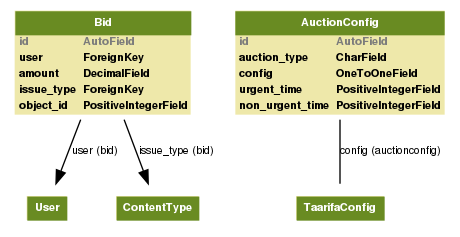
\includegraphics[scale=0.51]{img/auctions.png}
\caption{Figure to show UML diagram for the auctions app}
\label{fig:auc:uml}
\end{figure}

\subsubsection{Bid}
This class represents a bid a user makes. To make the auctions app as generic as possible, Bid uses a capability Django provides called GenericForeignKey. Ordinarily foreign keys must be defined on another model (Figure~\ref{lst:model}). Django's ContentType framework stores every defined model in a database table. GenericForeignKey uses this table to store pointers to the model ID and the instance ID, thereby enabling generic foreign keys. The API is not complete and there is a known bug in one of the methods which means additional code was written to bypass the bag. \\

\subsubsection{AuctionConfig}
This defines a one-to-one relation with TaarifaConfig which means that it will appear on the taarifa\_config admin page. \\

\begin{figure}
\centering

\includegraphics[scale=0.45]{img/bidform.png}
\caption{Figure to show the bid form}
\label{fig:bidform}
\end{figure}

\begin{figure}
\centering

\includegraphics[scale=0.45]{img/filterset.png}
\caption{Figure to show the filterset}
\label{fig:filter}
\end{figure}

The auctions app is designed to be pluggable. A programmer can implement a new auction by creating a Python module inside the auctions app. The AuctionConfig admin automatically detects this and presents the admin with a drop-down list, asking which type of auction they would like to run. In the future, it could be possible to allow them to run a different type of auction for urgent jobs. Alternatively, there could be a way to filter different jobs into different auctions. \\

For a programmer to plug into the auctions app, they must implement two view functions: view and bid; and provide a template ``bid.html" which contains the form to be displayed next to each job for a worker to bid on (Figure~\ref{fig:bidform}). When this form is submitted, the view in bid is called, and a programmer must implement this functionality. \\

View is passed the request object, a list of issues, a filterset, and a map. To enable the worker to filter the jobs, django-filter~\cite{filter} was installed. This provides a way to programmatically declare forms which the user can use to filter results on a page (Figure~\ref{fig:filter}). The list of issues passed to the view depends on the value provided by the GET request which is controlled by the filterset. The map is a plot of these facilities. \\